
% Revisado por Cristina el día 12/03/2013

\srsfuncion{Consultar plan de vuelo}
	Esta función muestra una formulario de búsqueda de vuelos y devolver al usuario una lista de vuelos introducidos anteriormente según sus restricciones para así obtener el plan de vuelo detallado de cada servicio.

	\begin{enumerate}
		\item \textit{Prioridad}: alta.
		\item \textit{Entradas}
		\begin{enumerate}
			\item Las opciones que admite el formulario de búsqueda son: \gls{numero_de_vuelo}, fecha y hora de origen y llegada, aeropuerto de origen y destino, y personal que forma parte de la tripulación.
			\item El número de vuelo caracteriza e identifica unívocamente a todos los vuelos operados por la compañía. Si dicho parámetro es introducido, todos los demás deben ser ignorados en la búsqueda. Se ha de comprobar que el formato del número de vuelo se corresponde con una sucesión de 4 caracteres numéricos (si el número de caracteres es menor que 4 se completará con \verb|0| por la izquierda).
			\item Las fechas y horas introducidas deben ser válidas.
			\item Los aeropuertos de origen y destino son un conjunto finito y han de haber sido configurados previamente. Internamente se componen de nombre, ciudad y código \gls{IATA}; externamente se visualizan como una secuencia de texto configurada. El usuario podrá seleccionar uno entre ellos para cada entrada (operación que se puede abreviar introduciendo el código IATA).
			\item En los circunstancias que se estime oportuno, aparecerá una lista editable de personal que formará parte de la tripulación del vuelo para filtrar resultados.
		\end{enumerate}
		\item \textit{Flujo de operaciones}
		\begin{enumerate}
			\item Se muestra un formulario con los campos anteriormente descritos.
			\item El usuario completa al menos uno de los diferentes campos. Ningún campo permite entradas erróneas por definición, salvo el de código de aeropuertos, que tras introducir un código de aeropuerto válido lo selecciona en el \gls{combobox} de aeropuertos y si no es válido no tiene efecto alguno, restaurándose su valor original.
			\item Si no se obtiene ningún resultado se informa de ello con un cuadro de diálogo. Si el resultado es único se muestra el plan de vuelo. Si se producen varias coincidencias se muestra una lista (indicando número de vuelo, fechas y aeropuertos) que permite la selección de alguno de ellos.
			\item Se accede a una nueva pantalla donde la información del plan de vuelo es distribuida de forma organizada. Desde esta pantalla se puede volver a la pantalla anterior de resultados y búsqueda.
		\end{enumerate}
		\item \textit{Respuesta a situaciones no previstas}
		\begin{enumerate}
			\item Si no se puede acceder a la base de datos de configuraciones, no mostrar la pantalla de inicio de la función e informar del error al usuario.
			\item Si la respuesta de búsqueda en la base datos no tiene lugar o es errónea, informar al usuario y permanecer en la pantalla actual como si no se hubiese buscado.
			\item Si la información de vuelos no puede ser obtenida, informar al usuario y permanecer en la pantalla actual como si no se hubiese buscado o seleccionado un vuelo.
			\item Si la información introducida en un plan de vuelo está dañada y no se puede acceder a ella, informar al usuario sobre lo sucedido y continuar en la pantalla actual para poder realizar otra búsqueda.
		\end{enumerate}
		\item \textit{Relación con otras funciones}
			Depende indirectamente de la función \verb|Introducir plan de vuelo|.
	\end{enumerate}

\begin{figure}[ht]\centering
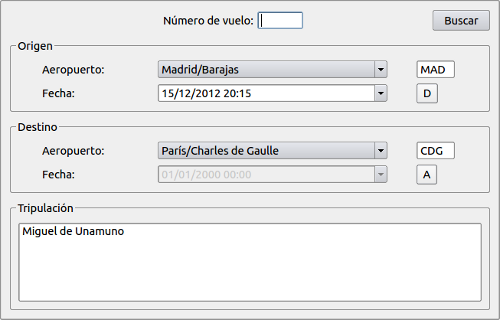
\includegraphics[scale=.6]{imagenes/BuscarPlanVuelo.png}
\caption{Pantalla aproximada de la búsqueda del plan de vuelo}
\end{figure}